\chapter{Background: Resource Estimations and Schedulers}
\label{Background.ch}

Data centers are among the largest energy consumers, accounting for approximately 4.4\% of total U.S. electricity usage in 2023, with projections suggesting an increase to 6.7\%–12\% by 2028, effectively tripling energy demands within the next three years \footnote{https://www.energy.gov/articles/doe-releases-new-report-evaluating-increase-electricity-demand-data-centers?utm_source=chatgpt.com}. Despite the rising power demands driven by AI workloads, an analysis of resource utilization on Ascend at OSC, a computing cluster primarily serving AI workloads, reveals that CPU-GPU utilization peaks at only 20–40\%, while memory utilization remains as low as 2–10\%. This substantial underutilization underscores a critical inefficiency, given the significant energy consumption required to maintain these systems. These findings emphasize the need for estimation frameworks that integrate with resource provisioning systems to enhance allocation strategies and optimize the utilization of shared clusters, ultimately improving energy efficiency in AI-driven data centers.

\section{Simple Linux Utility for Resource Management (SLURM)}
\label{sec:SLURM}
SLURM (Simple Linux Utility for Resource Management)\cite{jette2023architecture} is an open-source job scheduler widely used in high-performance computing (HPC) clusters, including data centers and academic supercomputers, for job scheduling and resource management. It offers a scalable and flexible framework for job submission, scheduling, and execution across distributed computing environments. SLURM partitions compute nodes into logical groups and manages job queues based on user-defined policies. It supports batch job scheduling, resource reservations, and fair-share scheduling, making it a preferred choice for supercomputing centers, research institutions, and enterprise HPC environments. Its plugin-based architecture allows customization for various scheduling strategies and integration with service management tools like TAPIS \cite{stubbs2021tapis}. With a lightweight and fault-tolerant design, SLURM ensures minimal overhead, making it ideal for large-scale scientific simulations, deep learning workloads, and complex parallel computing applications. 

\begin{figure}[ht]
    \centering
    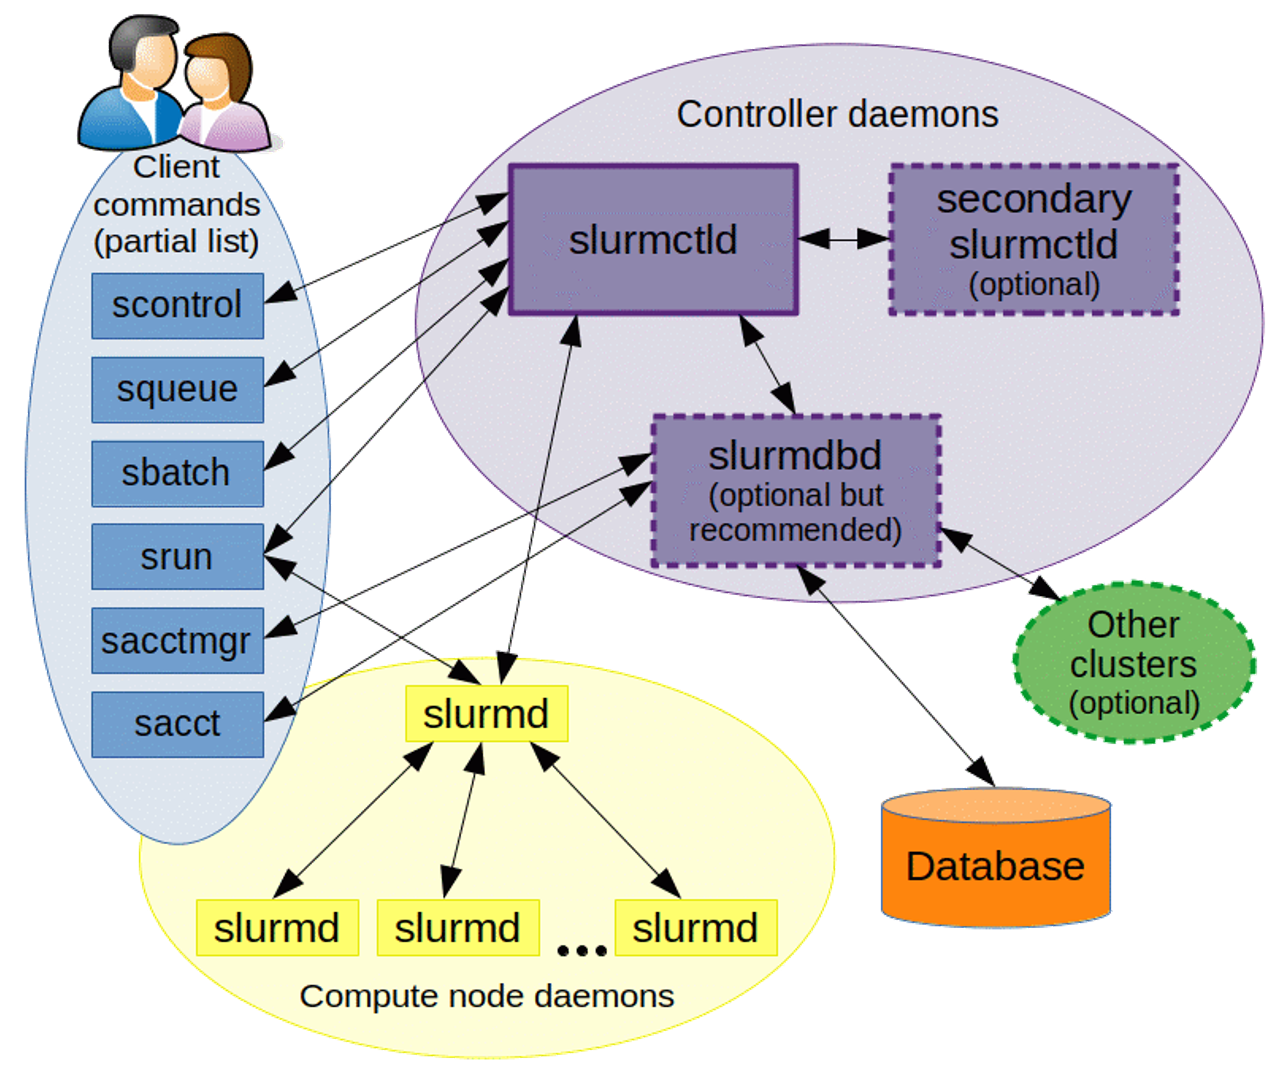
\includegraphics[width=\textwidth]{Images/SLURM.png}
    \caption{SLURM (Simple Linux Utility for Resource Management) Components}
    \label{fig:Slurm-Componenets}
\end{figure}

SLURM is composed of three primary components: the slurmctld (controller daemon), responsible for job scheduling, resource allocation, and queue management; the slurmd (compute node daemon), which runs on worker nodes to execute tasks and monitor resource usage; and the slurmdbd (database daemon), which integrates with an external database (e.g., MariaDB/MySQL) to store job accounting and usage data for historical tracking and reporting. Users interact with SLURM through command-line utilities such as sbatch (for submitting batch jobs), srun (for running interactive jobs), scancel (for canceling jobs), and squeue (for checking job status). End users specify job requirements in SLURM job scripts, defining parameters like CPUs, GPUs, memory, and execution time, while administrators manage partitions (logical groupings of compute nodes) and configure scheduling policies such as fair-share scheduling, preemption, and priority-based job execution. SLURM supports multiple scheduling algorithms, including first-come-first-serve (FCFS) and backfilling, ensuring efficient job placement based on resource availability. Its plugin-based architecture allows for seamless integration of custom scheduling policies and machine learning-driven resource prediction, making SLURM a key foundation for developing AI-driven schedulers and resource estimators that leverage its architecture for intelligent workload management \cite{tanash2021ensemble, okafor2024queue, ding2023mirage].

\section{Existing Resource Estimators}

Efficient resource provisioning can be achieved by optimizing several factors, including selecting the best execution endpoint based on resource requirements, estimating near-optimal allocations for successful workload execution, choosing scheduling algorithms that maximize overall utilization, reducing wait times, and improving energy efficiency. Figure \ref{fig:background_area} provides an overview of different estimation approaches that contribute to efficient, estimation-based resource allocation. It highlights the sources of training data and the types of estimators, such as black-box or white-box models and offline or online profiling methods. Most research focuses on estimating either wait time or execution time, as job staging time is theoretically constant and significantly shorter compared to wait times and execution times, particularly for computationally intensive workloads.

\begin{figure}[ht]
    \centering
    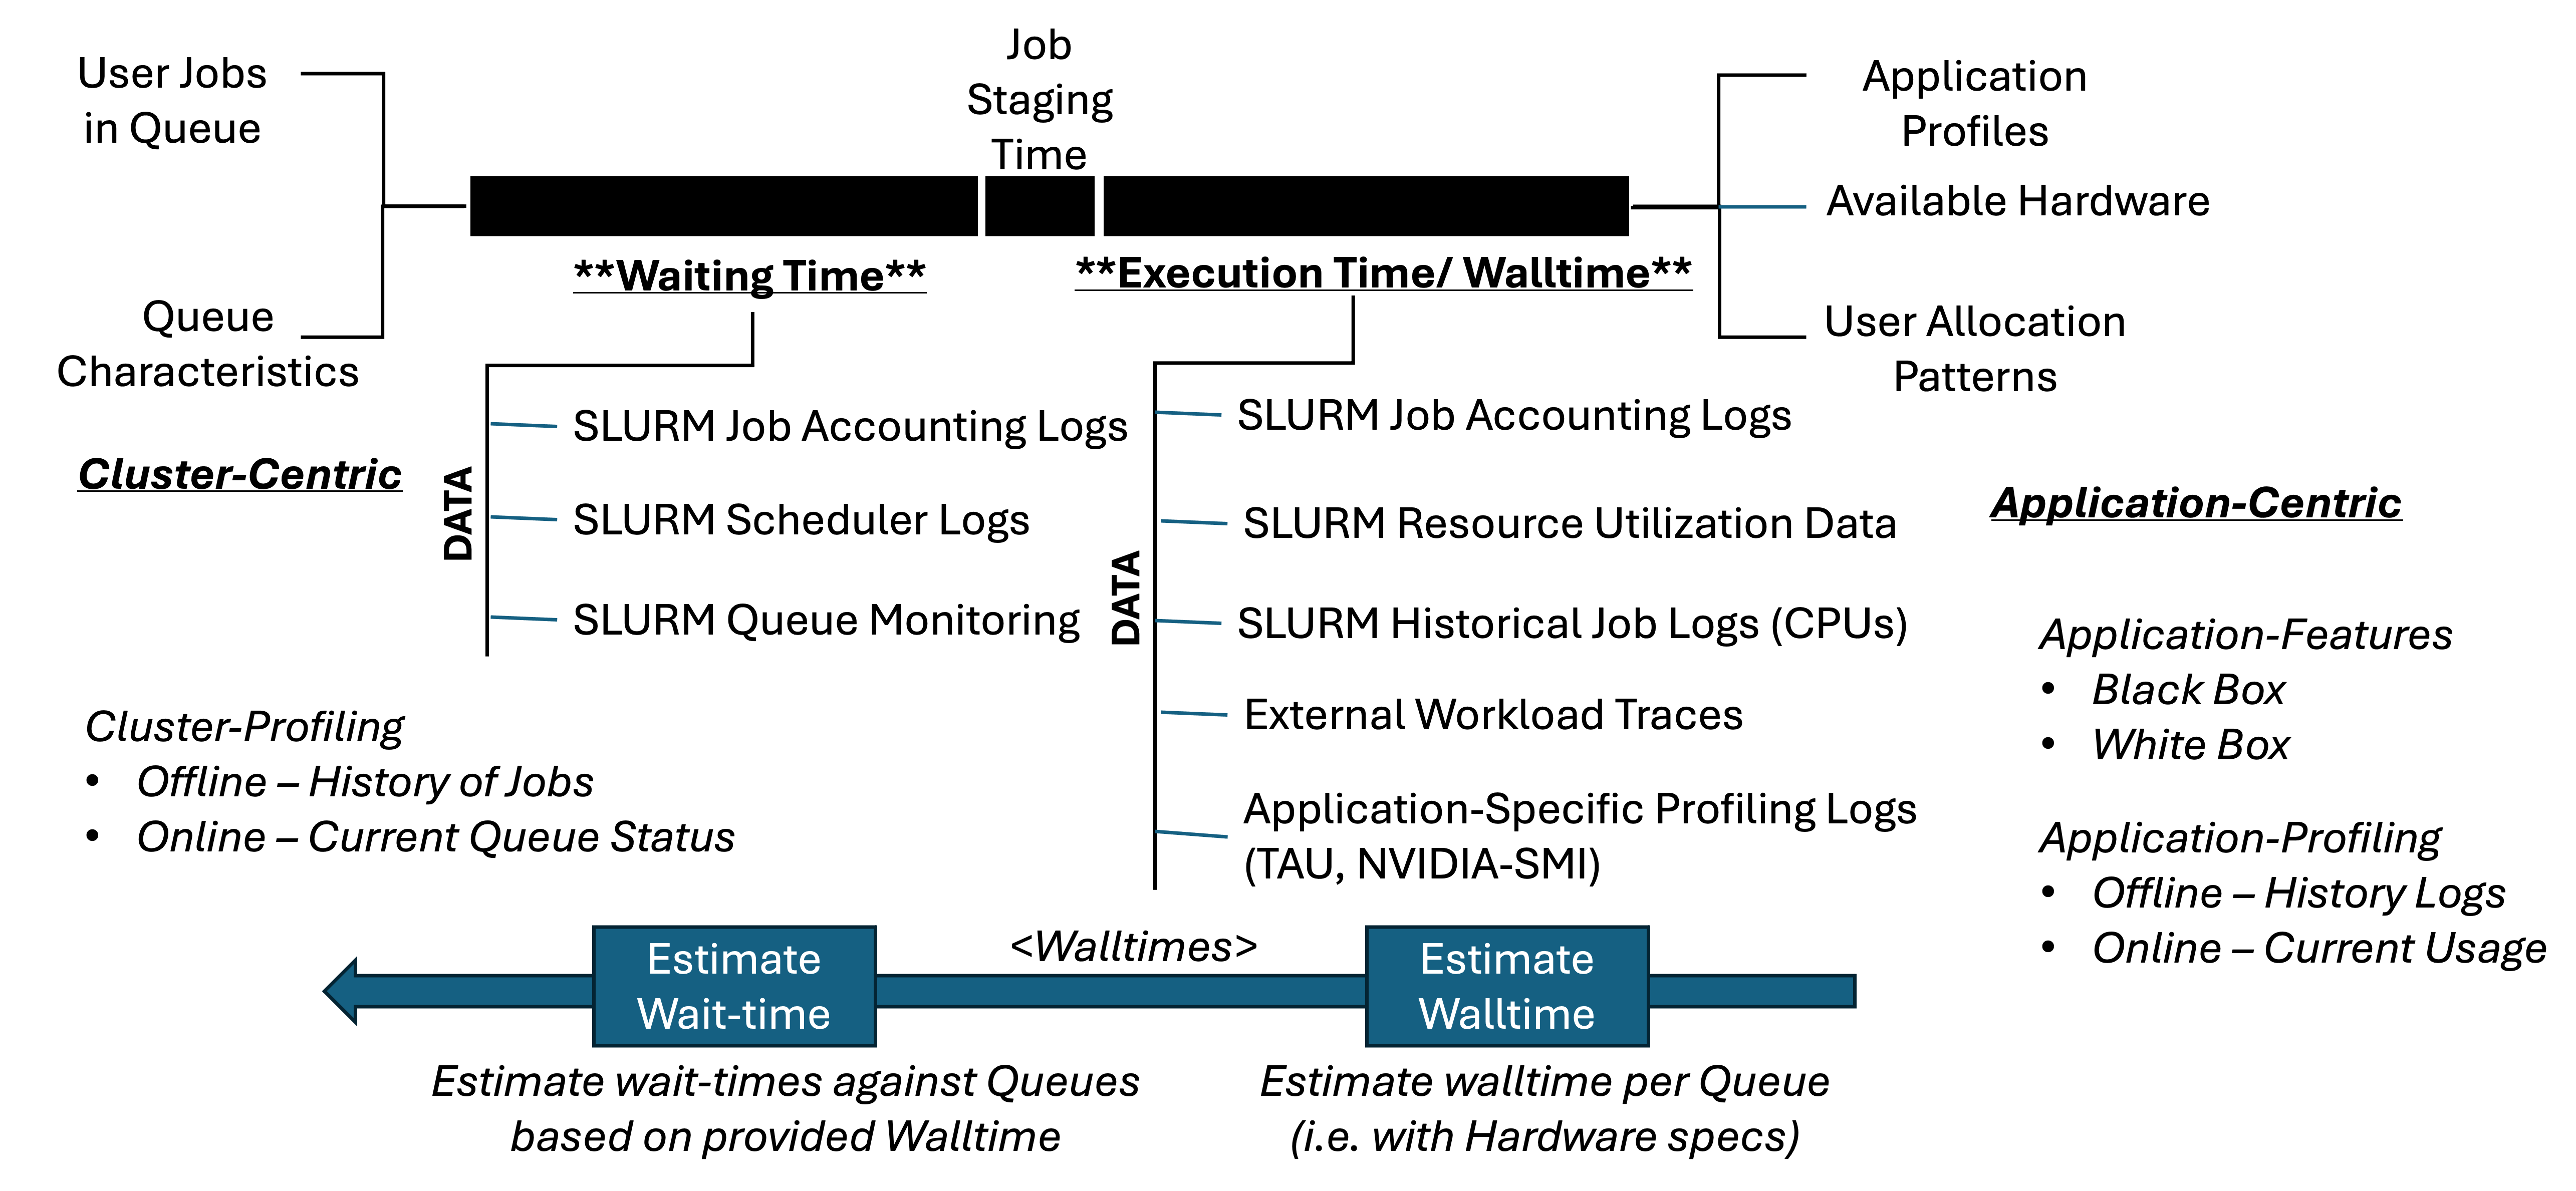
\includegraphics[width=\textwidth]{Images/Background_Area.png}
    \caption{An overview of different estimation approaches that contribute to efficient, estimation-based resource allocation}
    \label{fig:background_area}
\end{figure}

Some research focuses on streamlining wait time estimation \cite{okafor2024queue, brown2022predicting}, which heavily depends on SLURM logs and is specific to the cyberinfrastructure. Estimating wall times and execution times can also be approached from a user-centric perspective, particularly when researchers rely on a specific set of tools (e.g., Trimmomatic, SOAPdenovo) throughout their studies. These tools are frequently used in targeted domains such as genome sequencing. Alternatively, other approaches \cite{smartslurm2024, jaros2022optimization} take an application-centric view, focusing on understanding and estimating the resource demands of deep neural network workloads.

A range of online scheduling algorithms exist, some of which are cyberinfrastructure-agnostic \cite{venkataswamy2024launchpad}, while others are custom-tailored to specific CI environments to estimate wait times. In contrast, runtime estimators can be offline, online, or hybrid. Offline profilers rely on historical execution data to make predictions for future runs or emulate workflows on target environments before making estimations based on these emulations. Online estimators, on the other hand, start by executing a job with an initial configuration and refine predictions based on real-time performance, making them more suitable for pay-by-use models rather than traditional batch scheduling.

Hybrid approaches, such as predicting soft wall times \cite{chlumsky2022improving}, aim to refine runtime estimations dynamically. These methods begin by predicting an initial runtime that is shorter than the user-provided estimate, based on historical allocation utilization. The scheduler treats this as the initial allocation wall time and doubles it incrementally until the job either completes execution or reaches the user-provided runtime. Most resource estimators rely on SLURM log data, including user ID, queue, job submission time, job start time, total execution time, and other scheduling details, rather than actual application execution traces. Similarly, reinforcement learning algorithms are being explored for offline pre-training and online fine-tuning of scheduling strategies.

While some models use real job traces from supercomputing centers \cite{tanash2021ensemble, nakai2024node}, others rely on simulated data \cite{casanova2022feasibility, ohmura2022toward, ding2023mirage} due to data center policies restricting the sharing of job traces to protect user privacy and maintain data security. Additionally, the lack of diverse execution configurations in public datasets remains a challenge, as users often either use default configurations or repeatedly submit jobs with the same workable allocations.

Certain models treat runtime estimation as a classification problem \cite{reiner2016highly, klusavcek2024real}, rather than the traditional regression-based approach. Although many schedulers share a common feature space—including user ID, nodes, CPUs, GPUs requested, job submission time, job start and end time, and other SLURM job metadata—datasets are often not reusable across studies due to differences in hardware configurations and user workloads. Furthermore, some research papers do not publicly release the real SLURM workloads used to build their schedulers, citing data privacy concerns related to preserving user-HPC interactions.

\begin{itemize}
    \item Lack of Public Datasets – SLURM logs are often private, and queuing policies vary significantly across supercomputing centers, making it difficult to develop generalizable scheduling and resource estimation models.
    \item Stale Training Data – Cyberinfrastructure undergoes frequent changes, including hardware upgrades, middleware updates, and software modifications. Additionally, user workloads evolve rapidly, particularly in AI research, where deep neural network (DNN) architectures continuously adapt to newer and more efficient state-of-the-art (SOTA) models, either for improved accuracy or reduced model size. Existing traces, such as the MIT Data Center dataset \cite{fallon2013stata}, may no longer align with current workloads, limiting their applicability in modern research.
\end{itemize}

In contrast to scheduling-based predictors that rely on SLURM logs (whether real or synthetic), this thesis focuses on application-centric resource prediction. The primary objective is to estimate resource requirements based on the application itself, its parameters, and the available execution endpoints, rather than depending solely on historical SLURM logs. To reduce reliance on stale training data, this approach involves continuous profiling of applications against the current node configurations available in cyberinfrastructure (CI) systems. This ensures that estimations remain accurate and adaptable to evolving workloads and system architectures.

Chapter \ref{OverviewSolution.ch} presents various software stack solutions developed in this research to address the problems identified in Chapter \ref{problem.ch} and the limitations of existing approaches. While the proposed method focuses on generating application-centric training data through application execution profiling on targeted hardware, careful consideration is required to ensure that this process remains cost-efficient. Since emulating execution runs consumes valuable CI resources and adds to resource provisioning queues, an optimized approach is necessary. Chapter \ref{GenerateData.ch} explores a dual profiling methodology—"Scaled-Down" (SD) and "Full-Scale" (FS)—which balances profiling configurations with a human-in-the-loop feedback mechanism to generate training data while minimizing computational overhead efficiently. We also explore the development of a "Smart-Scheduling" framework inspired by SLURM, proposing the creation of a pre-SLURM CI database to enhance resource estimation and job execution. This database would serve multiple functions, including validating resource estimations against available queuing configurations, fetching hardware configurations to provide real-time input to inference estimators, and facilitating job execution. Additionally, we propose a job activation daemon that interacts with the database and resource estimators to generate an execution plan (batch submission), submit jobs, and track their progress until completion.
